% Copyright (c) 2013 Joost van Zwieten
%
% Permission is hereby granted, free of charge, to any person obtaining a copy
% of this software and associated documentation files (the "Software"), to deal
% in the Software without restriction, including without limitation the rights
% to use, copy, modify, merge, publish, distribute, sublicense, and/or sell
% copies of the Software, and to permit persons to whom the Software is
% furnished to do so, subject to the following conditions:
%
% The above copyright notice and this permission notice shall be included in
% all copies or substantial portions of the Software.
%
% THE SOFTWARE IS PROVIDED "AS IS", WITHOUT WARRANTY OF ANY KIND, EXPRESS OR
% IMPLIED, INCLUDING BUT NOT LIMITED TO THE WARRANTIES OF MERCHANTABILITY,
% FITNESS FOR A PARTICULAR PURPOSE AND NONINFRINGEMENT. IN NO EVENT SHALL THE
% AUTHORS OR COPYRIGHT HOLDERS BE LIABLE FOR ANY CLAIM, DAMAGES OR OTHER
% LIABILITY, WHETHER IN AN ACTION OF CONTRACT, TORT OR OTHERWISE, ARISING FROM,
% OUT OF OR IN CONNECTION WITH THE SOFTWARE OR THE USE OR OTHER DEALINGS IN
% THE SOFTWARE.
%
\documentclass{tudelftposter}

% optional, makes QR code clickable
\usepackage[hidelinks,implicit=false,bookmarks=false]{hyperref}

\usepackage{listings}
\lstset{basicstyle=\ttfamily\scriptsize,
  showstringspaces=false}

\title{Building complete free and open source GIS infrastructure for
  hydrological computing and data publication using GIS.lab and
  Gisquick platforms}

\addauthornote{mail}[@]{\ttfamily martin.landa@fsv.cvut.cz}
\addauthornote{diam}{Faculty of Civil Engineering, CTU in Prague}
\addauthornote{tp}[**]{OpenGeoLabs s.r.o., Czech Republic}

\addauthor[mail,diam]{M. Landa}
\addauthor[diam]{P. Kavka}
\addauthor[diam]{L. Strouhal}
\addauthor[tp]{J. Cepicky}

\addfootimage(c:right column.center)[Czech Technical University in Prague]{cvut}
\addfootqrcode(l:left column.left)[Derived from latex-poster-class]{https://github.com/tudelft-diam-na/latex-poster-class}

\begin{document}

\section{Introduction}

Building a complete open source GIS infrastructure allowing operations
from data preparation, analysis and computation to publishing results
to end-user is a very complex task. This poster presents GIS.lab as an
open source software solution which helps to build complete GIS
infrastructure in an easy, but still fully customized manner.

\section{GIS.lab as a Core Component}

% KAO: Remove spacing before label: can cause reference to be wrong
\begin{figure}[ht!]
\begin{center}
  
\includegraphics[width=.15\columnwidth]{../paper/figures/gislab-logo.png}
  \caption{GIS.lab logo (source: GIS.lab Documentation)}
\label{fig:gislab_logo}
\end{center}
\end{figure}

\noindent \textbf{GIS.lab} (\url{http://web.gislab.io}) has been
originally designed with a goal to enable simple, unbreakable
deployment of a complete, centrally managed, horizontally scalable GIS
infrastructure in the local network area (LAN), data center or cloud
in a few steps. GIS.lab is able to turn diverse open source GIS
software packages into a seamlessly integrated easy-to-use system. As
a result GIS.lab significantly decreases deployment of such complex
GIS infrastructure to absolute minimum, but still keeping the whole
technology under a full control of the system operator.

\section{Gisquick as a Publication Platform}

\textbf{Gisquick} (\url{http://gisquick.org}) is a separate project not
directly related to GIS.lab. It is a web application based on modern
technologies as Django, Angular and OpenLayers 3 with fully responsive
design optimized also for mobile devices. The main purpose of Gisquick
is to provide the capability for easy publishing the QGIS projects on
the web. 

\vskip 0.25in

% KAO: Remove spacing before label: can cause reference to be wrong
\begin{figure}[ht!]
\begin{center}
  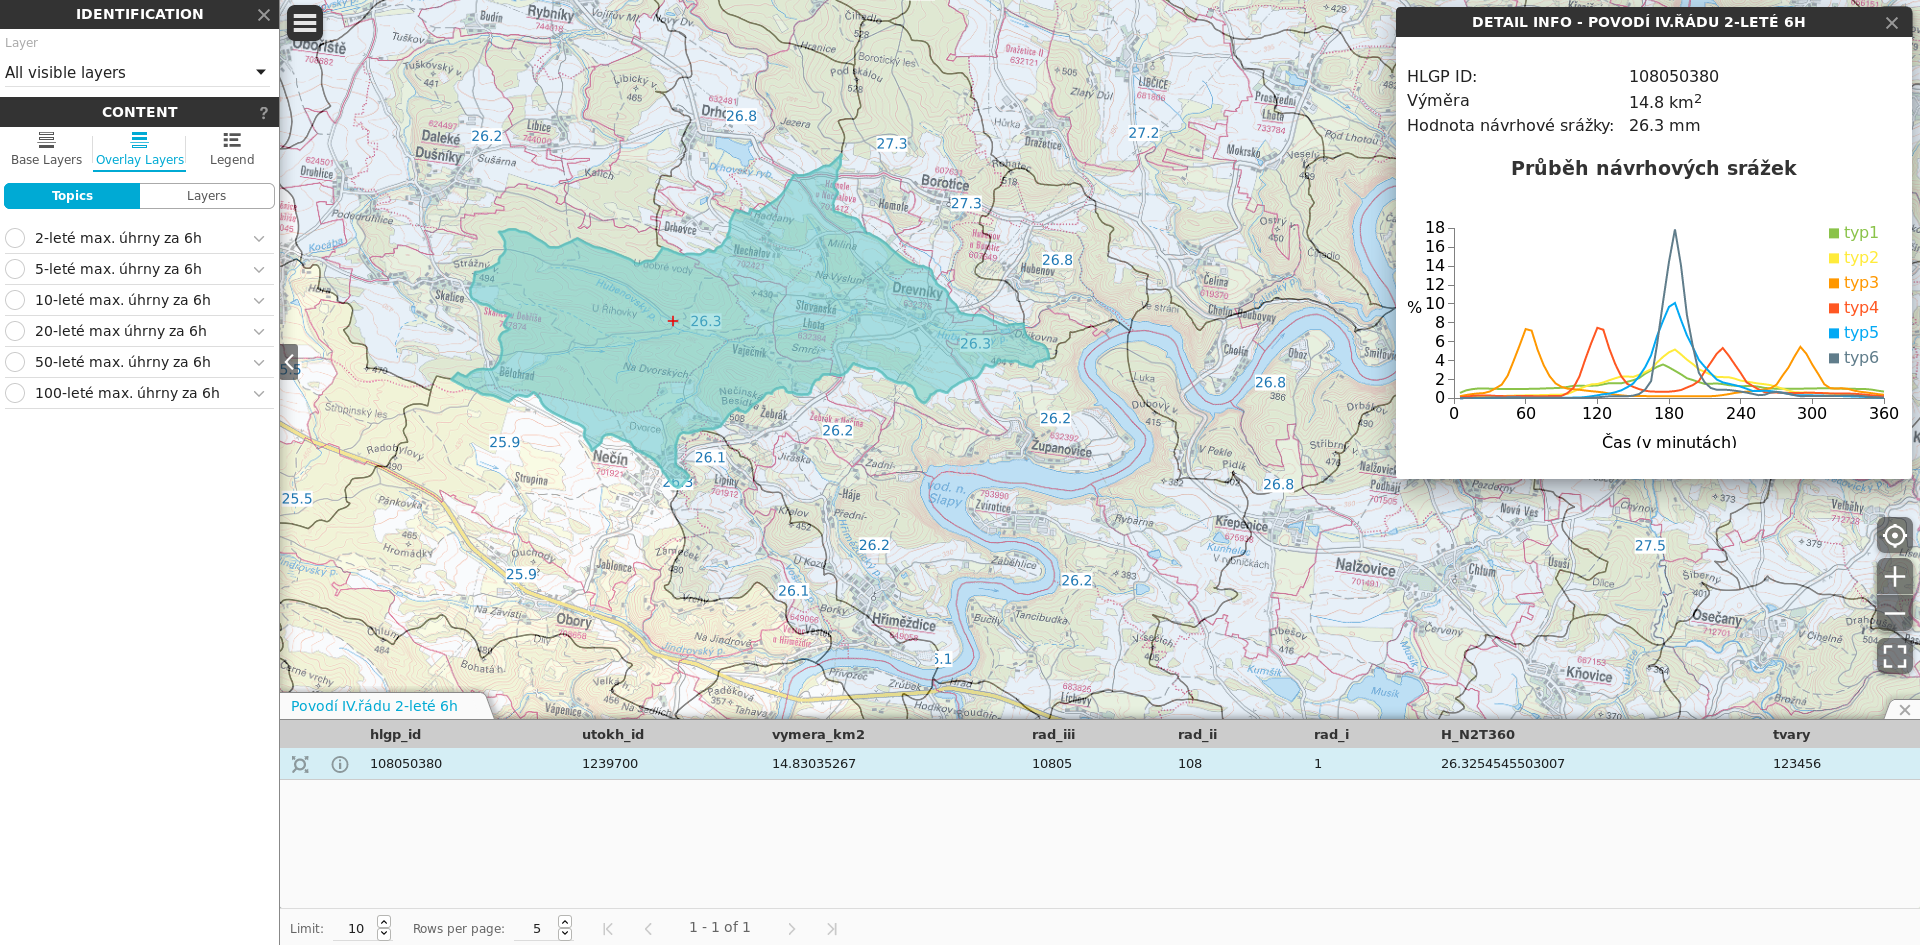
\includegraphics[width=0.85\columnwidth]{gisquick-example.png}
  \caption{Gisquick web application interface
    (source: author)}
\label{fig:gislab_infrastructure}
\end{center}
\end{figure}

\section{Case study}

Desired system should allow the user to collect, prepare, and
preprocess data from heterogeneous data sources for hydrological
computation using GIS software packages. The results of hydrological
data processing can be easily published via web services from user
desktop environment and ideally also as the interactive web mapping
applications provided by the server component (master node) in the
infrastructure.

Most of the requirements are already fulfilled by GIS.lab
platform. Missing features can be easily integrated into GIS.lab
eco-system by customizing the deployment of the both master/server and
desktop client components.

\vskip 0.4in

\noindent The procedure consists of \textbf{three major steps}:

\vskip 0.1in

\textbf{1. Deployment of  a Master Node}

Master node (playing a role of a server) of geospatial cluster can be
automatically deployed thanks to GIS.lab technology.

\vskip 0.1in

\textbf{2. Master Node Customization}

Customization rules are defined by \textit{Ansible Playbooks}
similarly how GIS.lab provision works. Example below demonstrates how
can be implemented a role for installing and configuring PyPWS4.

\begin{lstlisting}[numbers=left,xleftmargin=1em]
- name: Install PyWPS4
  pip:
    name: pywps
    version: 4.0.0

- name: Set up PyWPS4 configuration
  template:
    src: pywps.cfg.j2
    dest: /opt/pywps4/pywps.cfg
    mode: 0644
\end{lstlisting}

\vskip 0.1in

\textbf{3. Gisquick integration}

Gisquick project provides core \textit{Docker images} for successful
running of this publishing platform. It significantly simplifies
Gisquick integration into GIS.lab infrastructure. Docker images can be
automatically composed on GIS.lab master node by
\textit{docker-compose} command performed by customized provision
roles.

\section{Conclusions}

Combining GIS.lab and Gisquick technologies leads to a complete,
seamlessly integrated platform capable to prepare the input data,
perform geospatial analysis as services and publish results easily on
the web in the sense of interactive web mapping applications.

{\footnotesize \textbf{Acknowledgements} This work has been supported by the research
project QJ1520265 - "Variability of Short-term Precipitation and
Runoff in Small Czech Drainage Basins and its Influence on Water
Resources Management"}

\end{document}
% vim: tw=80:ts=2:sts=2:sw=2:et:fdm=marker:fmr=[[[,]]]
